\chapter{Codifica di linea}

\begin{figure}[h]
    \centering
    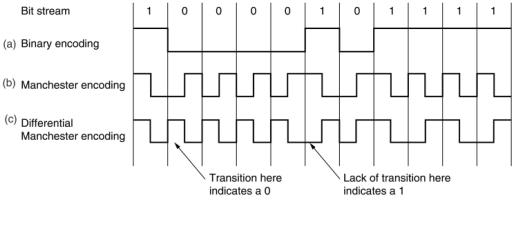
\includegraphics[scale = 1]{manchester_coding1.jpg}
\end{figure}

\newpage 

\section{Cosa è la codifica di linea}
\footnote{Slide del prof | Codifica di linea | pag 1 \\  
Slide | Codifica di linea | pag  1\\
Appunti | 2025-03-25 | pag 2 - 3
}

In un mezzo trasmissivo, l'informazione è contenuta alle alte frequenze, 
perchè le basse frequenze, generalmente, vengono alterate dal mezzo trasmissivo stesso. \newline 

Data una sequenza di bit come la seguente: 

{
    \Large 
    \begin{equation}
        0101100
    \end{equation}
}

in cui ogni bit (ad esempio il primo bit della sequenza che è lo 0) 
verrà trasmesso in un tempo $T_b$. \newline 

Allora la frequenza di trasmissione è l'inverso di $T_b$, cioè $f_0$: 

{
    \Large 
    \begin{equation}
        f_0 = \frac{1}{T_b}
    \end{equation}
}

L'obiettivo di qualsiasi trasmissione in un mezzo trasmissivo è quello di inviare più bit utilizzando la larghezza di banda più piccola possibile 
(specialmente quando si tratta di inviare bit nelle comunicazioni wireless dove lo spettro è limitato e non bisogna interferire con gli altri utenti). \newline 

Inoltre, la scelta del tipo di forma d'onda da adottare per la trasmissione numerica può essere condizionata, 
oltre dalla necessità di controllare l'interferenza di intersimbolo (o ISI) e di minimizzare la probabilità di errore anche da diverse esigenze. \newline 

\begin{tcolorbox}
    Riguardo alla probabilità di errore, è un argomento che verrà trattato in seguito in queste pagine. \newline 

    Per quanto riguarda l'ISI, ne avevamo già discusso nel corso precedente di Teoria dei segnali. \newline 

    Un piccolo ripasso: \newline 

     \url{https://github.com/ciccio25/appunti-teoria-dei-segnali/blob/main/Appunti%20Teoria%20dei%20segnali.pdf} \\
    Capitolo 11 - Interferenza di intersimbolo - pag 101 - 108
\end{tcolorbox}

Problemi tipici (ma non esclusivi) riguardo alla scelta del tipo di forma d'onda in un canale sono: 

\begin{itemize}
    \item necessità di minimizzare il contenuto spettrale del segnale alle basse frequenze 
    \item necessità di semplificare l'operazione di sincronizzazione in ricezione
\end{itemize}

\begin{tcolorbox}
    Il primo punto è banale perchè, essendo alle basse frequenze, lo spettro è decisamente limitato rispetto ad andare ad alta frequenza, dove il segnale, in frequenza, è molto più largo. \newline 

    Il secondo punto non verrà affrontato in questo corso. \newline 

    Il problema della sincronizzazione è un problema gigantesco da affrontare nella teoria dell'informazione. \newline 

    L'unica cosa che dobbiamo sapere al momento è che, se non c'è una sincronizzazione tra gli apparati nelle trasmissioni digitali, 
    gli zeri e uni che gli apparati ricevono vengono interpretati come simboli "a caso, senza senso, senza contenuto informativo" piuttosto che essere utili e informativi. 
\end{tcolorbox}


La procedura che conduce alla definizione della migliore forma d'onda per il particolare sistema o canale considerato, 
prende il nome di "codifica di canale". \newline 

\newpage 

\subsection{Segnali unipolari: NRZ e RZ}
\footnote{Slide del prof | Codifica di linea | pag 1 - 2\\  
Slide | Codifica di linea | pag  1 - 2\\
Appunti | 2025-03-25 | pag 4
}

Assumiamo come riferimento il caso di trasmissione di dati binari (0 e 1) di durata T. \newline 

Una prima scelta che si impone è se trasmettere il segnale in forma unipolare o bipolare. \newline 

Nel caso unipolare, il segnale sarà costituito da una sequenza di livelli alti (che indicheremo con V o +V) e di livelli bassi (che indicheremo con 0), 
mentre nel caso bipolare comparirà, oltre al livello +V e 0, anche il livello -V. \newline 

Riferendoci al caso unipolare, sono peraltro possibili due soluzioni. \newline 

La prima soluzione di caso unipolare è denominata come NRZ (Non Return to zero) dove il singolo bit di informazione viene trasmesso utilizzando un impulso rettangolare, di durata T e di ampiezza V 
quando il bit vale 1; se il bit vale 0 viene trasmesso un segnale di ampiezza nulla di durata T. \newline 

Un esempio di segnale NRZ confrontato con il segnale di clock: 

\begin{figure}[h]
    \centering
    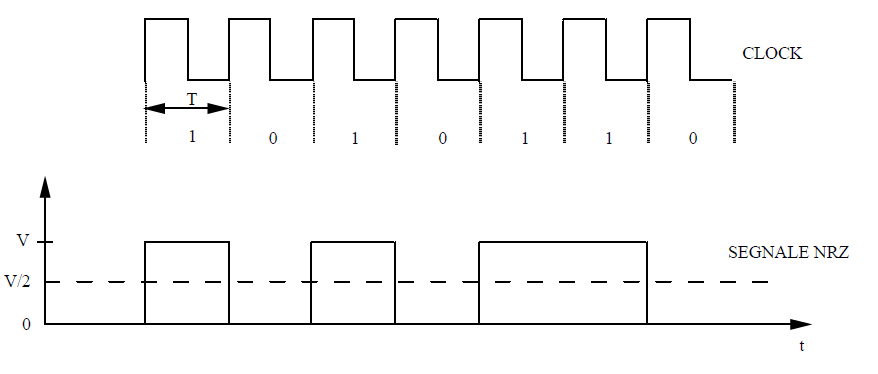
\includegraphics[scale = 1]{Segnale NRZ confrontato con il segnale di clock.PNG}
\end{figure}

Come si può visualizzare dall'andamento del segnale NRZ e la sequenza di bit sotto al segnale di clock, 
si possono avere variazioni del segnale solo alla fine di un intero periodo di clock. \newline 

Questo fatto ha implicazioni sullo spettro di potenza del segnale stesso, 
che risulta, in questo caso, proporzionale a $\left[ \frac{\sin(\pi \cdot f \cdot T)}{\pi \cdot f \cdot T}\right]^{2}$, 
oppure, detto a parole, è proporzionale a un sinc al quadrato. \newline 

\newpage 

\begin{tcolorbox}
    La funzione sinc la avevamo scoperta anche nel corso precedente. \newline 

    Per rinfrescare le idee, questo è l'andamento di un sinc: 

    dove il sinc in blu è normalizzato, mentre il sinc in rosso è un sinc non normalizzato. \newline 
    
    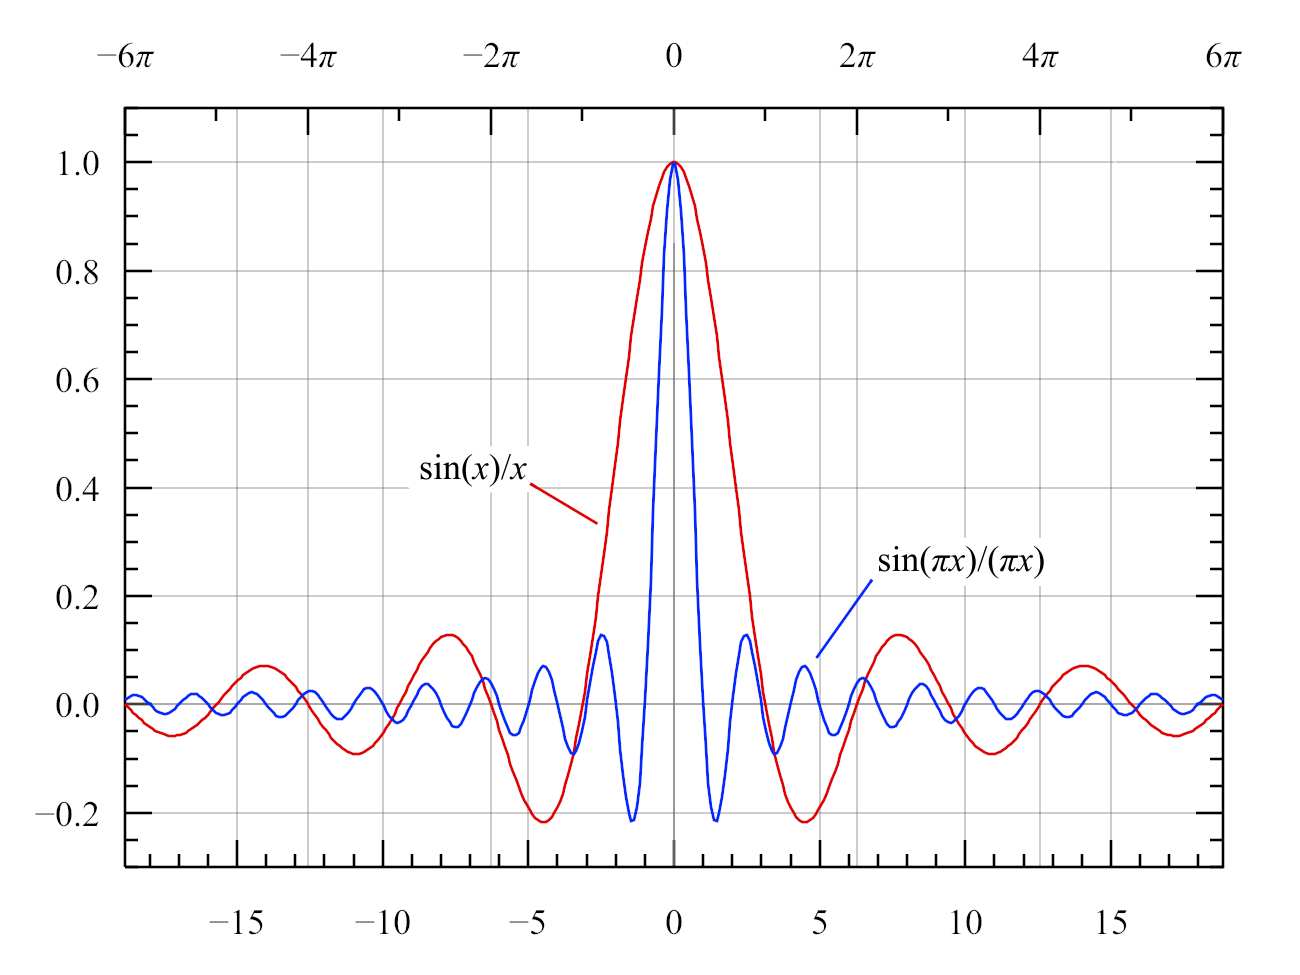
\includegraphics[scale = 1]{Sinc_function_(both).png}
    
    Per approfondire: \newline 
    \url{https://it.wikipedia.org/wiki/Funzione_sinc}
\end{tcolorbox}

Di seguito, lo spettro di potenza del segnale NRZ in frequenza normalizzato (con gli appunti presi a lezione): 


\begin{figure}[h]
    \centering
    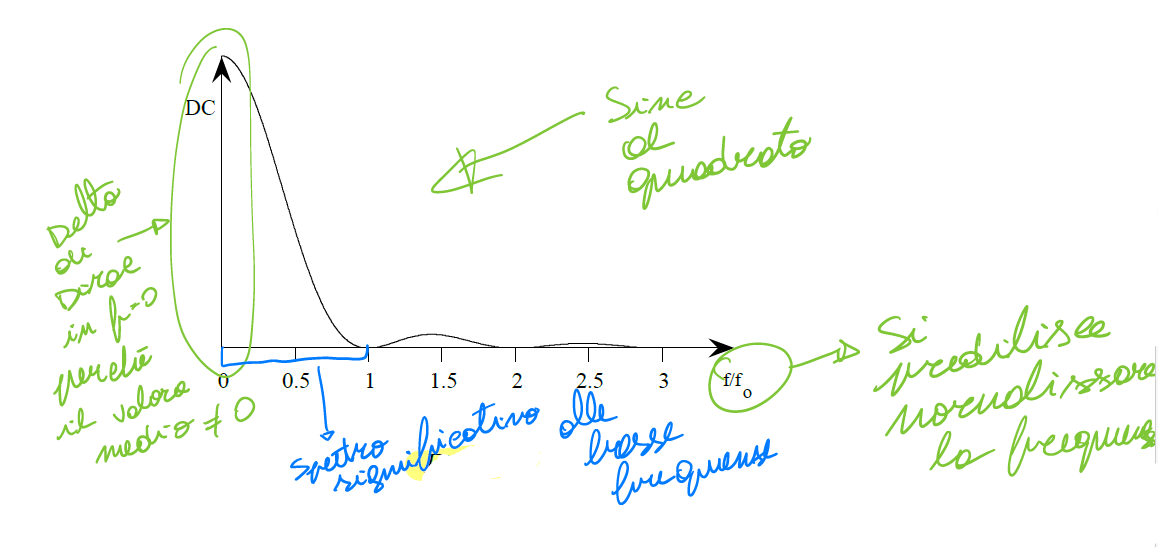
\includegraphics[scale = 0.7]{Spettro di potenza di un segnale NRZ.PNG}
\end{figure}

\begin{tcolorbox}
    Confrontando la figura del sinc e quella del sinc al quadrato, notiamo che gli andamenti negativi, 
    grazie all'elevamento alla potenza, sono diventati positivi e, siccome si considerano andamenti con il tempo maggiore di zero, 
    il sin al quadrato viene "tagliato" a metà, viene presa solo la metà a destra.  

\end{tcolorbox}

In figura si è posto: 

{
    \Large 
    \begin{equation}
        f_0 = \frac{1}{T}
    \end{equation}
}

Il lobo principale dello spettro in frequenza di un segnale NRZ ha spettro uguale a $f_0$, 
e si hanno valori nulli in corrispondenza di multipli di $f_0$, detta anche frequenza fondamentale. \newline 

Inoltre è presente la Delta di Dirac nell'origine perchè il segnale ha valore medio diverso da zero, 
che ha valore $\frac{V}{2}$. \newline 

Viene chiamata come NRZ (Non Return to Zero) perchè il bit 1 non diventa mai 0 [V]. \newline 

Invece di seguito l'andamento nel tempo di una codifica RZ (Return to Zero) confrontato con il segnale di clock: 

\begin{figure}[h]
    \centering
    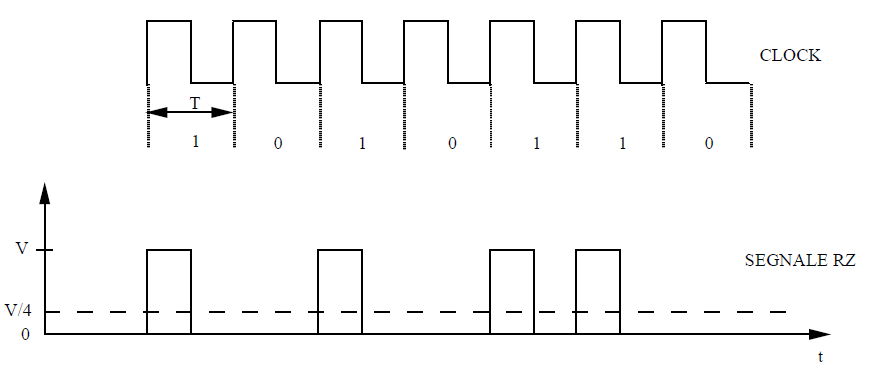
\includegraphics[scale = 0.8]{Segnale RZ e clock.PNG}
\end{figure} 

con il suo spettro di potenza in frequenza normalizzato: 

\begin{figure}[h]
    \centering
    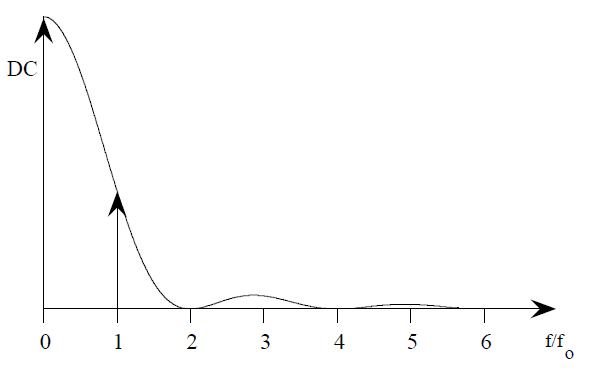
\includegraphics[scale = 0.8]{Spettro di potenza in frequenza del segnae RZ.PNG}
\end{figure} 

Notando il segnale di RZ nel tempo, la trasmissione del livello V è limitata a mezzo intervallo di simbolo, cioè $\frac{T}{2}$. \newline 

In pratica, si può avere una transizione del segnale ogni $\frac{T}{2}$ secondi. \newline 

Lo spettro spettro di potenza, come il caso dell'NRZ, risultato proporzionale al sinc al quadrato, cioè $\left[ \frac{\sin(\pi \cdot f \cdot T)}{\pi \cdot f \cdot T}\right]^{2}$, 
e ciò ha conseguenza un allargamento del lobo principale. \newline 

\begin{tcolorbox}
    Molto importante è la relazione tra tempo e frequenza. \newline 

    Sembra banale, ma ripassiamola al momento. \newline 

    Se abbiamo un segnale nel tempo con transizioni lente, si avrà un andamento in frequenza molto stretto. \newline 

    Se abbiamo un segnale nel tempo con transizione molto rapide, si avrà un andamento in frequenza molto largo. \newline 

    Essendo la frequenza l'inverso del tempo, bisogna considerare che il comportamento del segnale nel tempo è inverso in frequenza.
\end{tcolorbox}

Quindi, rispetto al caso NRZ, il lobo principale non si estende fino a $f_0$, bensì fino a $2 \cdot f_0$. \newline 

I valori nulli sono presenti in valori multipli del lobo principale. \newline 

Essendo il valore medio del segnale NRZ nel tempo di $\frac{V}{4}$, avremo, in frequenza, una Delta di Dirac in continua. \newline 

Inoltre, sono presenti delle Delte di Dirac in presenza di frequenze dispare multipli di $f_0$ (in figura non sono mostrati, ma è presente una Delta di Dirac anche in $\frac{f}{f_0} = 3$ e in $\frac{f}{f_0} = 5$). \newline 

\newpage 

\subsubsection{Confronto spettro di potenza tra NRZ e RZ}
\footnote{Slide del prof | Codifica di linea | pag 2 \\ 
Slide | Codifica di linea | pag  2\\ 
Appunti | 2025-03-25 | pag 5
}

Dal confronto del segnale dello spettro di frequenza dell'NRZ e dell'RZ: 

\begin{figure}[h]
    \centering
    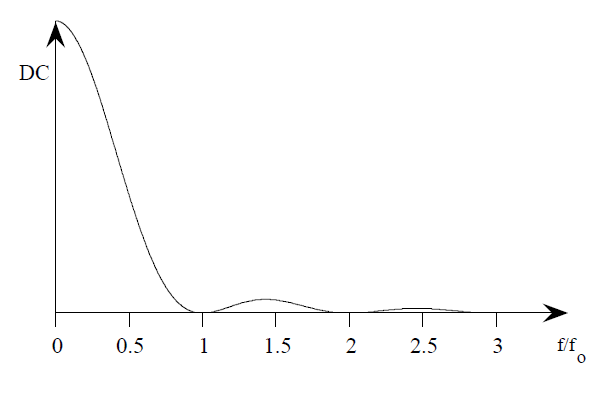
\includegraphics[scale = 0.8]{Spettro di frequenza di potenza di un segnale NRZ.PNG}
    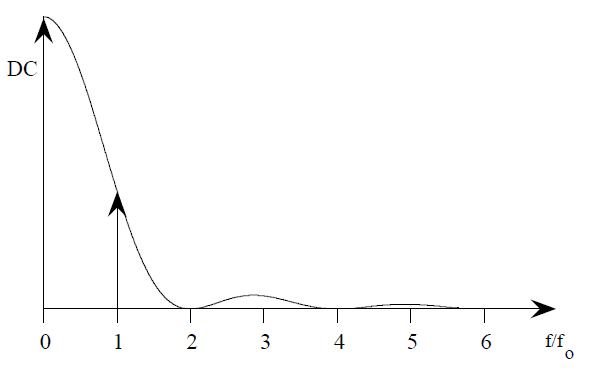
\includegraphics[scale = 0.8]{Spettro di potenza in frequenza del segnae RZ.PNG}
\end{figure} 

dove, la figura in alto è lo spettro di potenza di un segnale NRZ, 
e in basso è lo spettro di potenza di un segnale RZ. \newline 

Si nota che, nella soluzione NRZ, non si ha potenza alla frequenza $f_0$, 
a differenza dello spettro dell'RZ, in cui in $f_0$ è presente una Delta di Dirac. \newline 

Questa osservazione è importante perchè consente al ricevitore di concludere che la frequenza di clock può essere recuperata dal segnale trasmesso nel caso RZ (utilizzando un filtro passa-banda molto stretto limitato a $f_0$), 
mentre non è recuperabile nel caso NRZ. \newline 

La disponibilità della frequenza di clock (vale a dire della frequenza di trasmissione dei simboli binari) 
è importante in ricezione per poter sincronizzare gli apparati di rivelazione. \newline 

Per quanto detto, utilizzando lo schema NRZ, 
la frequenza di clock deve essere rigenerata localmente (quindi, dal punto di vista economico, bisogna avere un ricevitore con un oscillatore locale e tutti i componenti che gli stanno intorno), 
invece nel caso RZ può essere estratta dal segnale ricevuto (realizzare un filtro è nettamente più economico che aggiungere un oscillatore locale, anche perchè quest'ultimo è instabile e va termostatato, quindi un casino). \newline 

Ricordiamo uno tra gli obiettivi della codifica di linea, che è quello di semplificare l'operazione di sincronizzazione in ricezione: 
per questo motivo, la codifica RZ risulta normalmente preferibile rispetto a quella NRZ. \newline 

\newpage 

\subsection{Codifca AMI}
\footnote{Slide del prof | Codifica di linea | pag 3 - 4\\
Slide | Codifica di linea | pag  3 - 4\\  
Appunti | 2025-03-25 | pag 5 - 6
}

Sia nel caso NRZ che in quello RZ, il segnale ha un contenuto spettrale significativo alle basse frequenze (e in particolare un valor medio diverso da zero). \newline 

Ciò risulta svantaggioso in pratica. \newline 

Infatti, la componente continua, e più in generale le basse frequenze, vengono quasi sempre bloccate o distorte (si pensi ad un semplice condensatore presente in un circuito che, idealmente, blocca la continua). \newline 

Molte sono le tecniche di codifica utilizzabile per spostare lo spettro di potenza a frequenze più elevate. \newline 

Un esempio di tecnica senza la componente continua è la codifica AMI (Alternate Mask Inversion). \newline 

Un esempio di andamento di un segnale AMI nel tempo e del suo spettro di potenza in frequenza normalizzato a $f_0$ è il seguente (con le note): 

\begin{figure}[h]
    \centering
    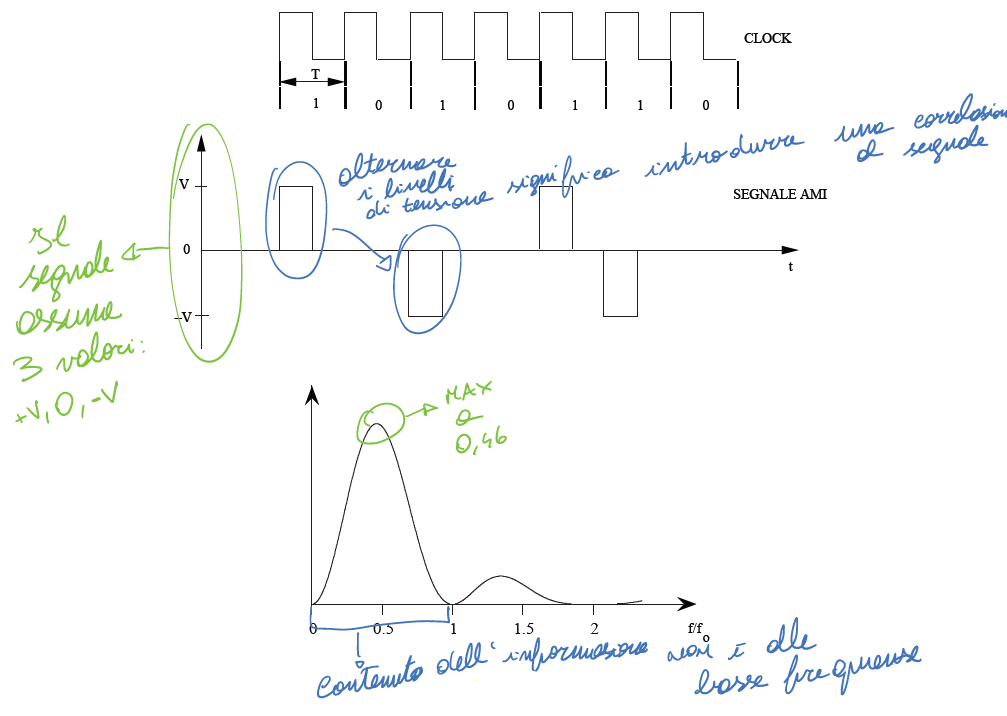
\includegraphics[scale = 0.85]{Andamento nel tempo di una codifica AMI e del suo spettro in frequenza di potenza.PNG}
\end{figure} 

Come si visualizza dalle seguenti figure, nella codifica AMI il simbolo 1 (ma la scelta è chiaramente convenzionale) 
viene alternativamente trasmesso il livello +V ed il livello -V nel tempo. \newline 

Inoltre, il segnale AMI è un segnale a 3 livelli: +V, -V e 0. \newline 

Come la codifica RZ, il segnale AMI può avere una variazione ogni $\frac{T}{2}$ secondi. \newline 

Inoltre, lo spettro di potenza in frequenza risulta diverso rispetto alla codifica NRZ e RZ. \newline 

L'alternanza nel tempo di +V e -V fa sì che il valor medio del segnale sia nullo (quindi non è presenta una Delta di Dirac in continua), 
inoltre il lobo principale è centrato su $0.46 \cdot f_0$ (cioè circa $\frac{f_0}{2}$). \newline

L'apparente mancanza della componente a frequenza $f_0$ può essere compensata semplicemente invertendo gli impulsi negativi nel tempo in ricezione, 
in tal modo ottenendo di nuovo il segnale in codifica RZ. \newline 

Così facendo, lungo il canale si trasmette il codice AMI (con i vantaggi che ciò comporta), 
mentre in ricezione, dove non si hanno più problemi di distorsione delle componenti a bassa frequenza, 
si utilizza il segnale RZ, con ciò semplificando l'operazione di sincronizzazione. \newline 

Un'altra caratteristica interessante del codice AMI è che si tratta di un codice capace di rivelare la presenza di errori. \newline 

Se il rumore sovrapposto al segnale trasforma un livello 0 in un livello +V o -V, 
si verifica certamente una violazione del codice (si avranno infatti due livelli +V o due livelli -V consecutivi), 
che consente di identificare la presenza dell'errore. \newline 

La stessa considerazione vale se il rumore trasforma un livello +V o -V in un livello 0. \newline 

Se il ricevitore ha solo la codifica AMI, il ricevitore può capire (o rivelare) se c'è stato un errore, 
ma (con le conoscenze che sappiamo adesso) non sa correggerlo, 
quindi, l'unica cosa che può fare il ricevitore, è richiedere la ritrasmissione del segnale. \newline 

\newpage 

\subsection{Codifica HBDn}
\footnote{Slide del prof | Codifica di linea | pag 4 \\
Slide | Codifica di linea | pag  4\\  
Appunti | 2025-03-25 | pag 6
}

Nello schema RZ, il recupero del sincronismo è possibile solo a condizione che non si abbiano in trasmissione lunghe sequenze di zeri. \newline 

Laddove si verifichi quest'ultima eventualità, infatti, il segnale trasmesso rimane costante per un lungo periodo di tempo e, non avendosi variazioni in ricezione, 
la frequenza $f_0$, non può essere rivelata. \newline 

Questo importante inconveniente può essere compensato ricorrendo ad altri schemi di codifica di linea. \newline 

Il più noto tra tutti è lo schema HDBn (High Density Bipolar di ordine n), 
dove n è un numero intero. \newline 

Utilizzando per la trasmissione del segnale numerico questo codice di linea, 
non è possibile avere più di n simboli nulli consecutivi nella sequenza di segnale. \newline 

L'eventuale (n + 1)-esimo livello 0, viene infatti sostituito "artificialmente" con un livello $\pm$V, 
ove la scelta del segno viene fatta violando intenzionalmente la regola dell'alternanza propria del codice AMI, 
per rendere possibile, in assenza di errori, l'identificazione. \newline 

Un esempio di un andamento nel tempo di codice HDB3 (cioè $n=3$, quindi non si possono avere più di 3 simboli nulli) 
è il seguente (con gli appunti presi a lezione): 

\begin{figure}[h]
    \centering
    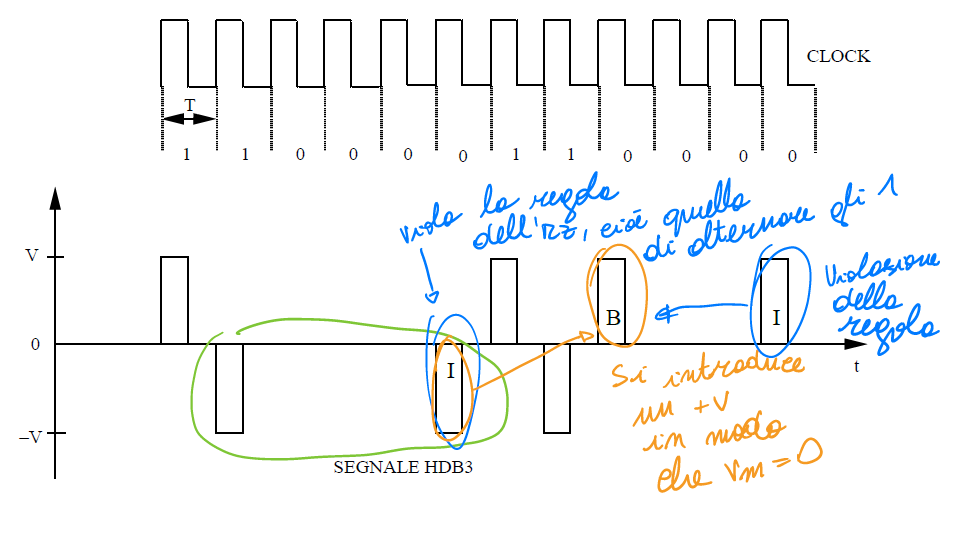
\includegraphics[scale = 0.9]{Segnale HDB3 con appunti.PNG}
\end{figure} 

La figura della HDB3 consente anche di specificare meglio le caratteristiche del codice 
in cui ogni violazione (indicate con 1 in figura) deve avvenire con cambiamento di polarità. \newline 

Se ciò non è possibile "naturalmente", allora il primo zero nella sequenza di quattro simboli nulli deve, 
a sua volta, essere trasformato in un 1. \newline 

In figura, il livello contrassegnato con B è stato forzato a +V, pur corrispondendo ad un simbolo 0, 
proprio per avere l'inversione di polarità nell'ultimo livello della seconda sequenza. \newline 

Così facendo, il valore medio del segnale resta circa uguale a zero, e, globalmente, lo spettro in frequenza della potenza del codice HDB3 è pressoché analogo al codice AMI. \newline 

\newpage 

\subsection{Altri codici di linea}
\footnote{Slide del prof | Codifica di linea | pag 5 - 6\\  
Slide | Codifica di linea | pag  5 - 6\\
Appunti | 2025-03-25 | pag 6 - 8
}

Codici di linea più complessi, come quelli della famiglia mBnT, 
trasformano m-uple di cifre binarie in ingresso in n-uple di cifre ternarie da trasmettere utilizzando tre livelli sulla linea, 
di cui anche qui uno a 0 e gli altri due con valore $\pm$V. \newline 

I codici della famiglia mBnT (come puri quelli HDBn) introducono, generalmente, 
una penalizzazione dal punto di vista della potenza necessaria per avere una certa quantità di trasmissione. \newline 

Per questo motivo, il loro uso è spesso combinato con quello di opportuni codici di canale. \newline 

Allo stesso tempo, però, l'occupazione spettrale che essi richiedono, quando n è minore di m, 
è di norma minore, e quindi il loro uso è consigliato nelle applicazioni in cui è fondamentale limitare la banda occupata. \newline 

Una diversa "filosofia" nell'ottica di risolvere il problema delle lunghe sequenze di simboli nulli, 
consiste nell'assegnare a ciascun simbolo binario una forma d'onda che presenta comunque variazioni all'interno dell'intervallo T. \newline 

L'esempio più significativo è costituito dal "codice bifase" (comunemente noto come "codice Manchester"). \newline 

\newpage 

Come mostrato nella seguente figura: 

\begin{figure}[h]
    \centering
    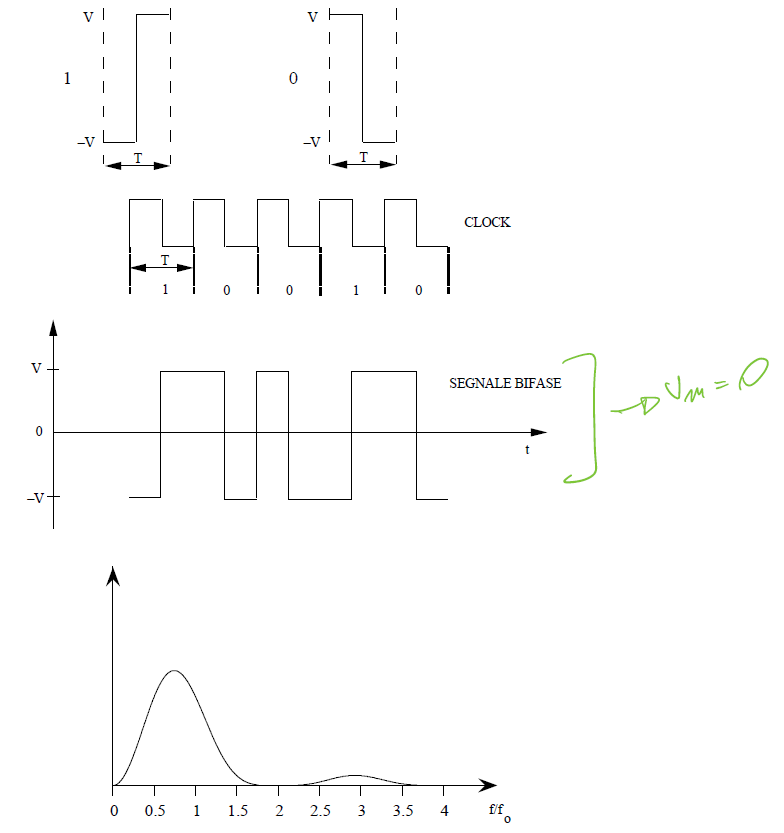
\includegraphics[scale = 1]{Codice Manchester.PNG}
\end{figure} 

nel codice Manchester si associa a ciascun bit una forma d'onda di valor medio nullo, di segno positivo o negativo a seconda del valore del bit. \newline 

Così facendo, il segnale presenta comunque una transizione a metà dell'intervallo di bit, e si ha transizione anche all'inizio dell'intervallo quando i due bit adiacenti sono identici. \newline 

Notando l'andamento dello spettro del codice Manchester, $f_0$ è certamente recuperabile, anche se, 
rispetto agli altri codice, l'assenza di una Delta di Dirac in $f_0$ rende un po' più sofisticato il recupero del sincronismo. \newline 

\newpage 

\section{Cenni sul problema della sincronizzazione}
\footnote{Slide del prof | Codifica di linea | pag 7 - 8\\
Slide | Codifica di linea | pag  7 - 8\\  
Appunti | 2025-03-25 | pag 8 
}

Per una corretta ricostruzione dell'informazione al ricevitore, 
è necessaria la conoscenza della frequenza di simbolo (cioè il clock visto nelle sezioni precedenti). \newline 

L'inverso di quest'ultima, infatti, vale a dire la durata T di ciascun simbolo, 
determina la distanza tra due istanti di lettura e di decisione successivi. \newline 

Il problema viene qui accennato con riferimento alla trasmissione numerica in banda base, 
ma un problema analogo si pone ovviamente anche nelle trasmissioni in modulazione (che verranno trattate successivamente nel corso). \newline 

Come si è visto in precedenza, con alcune tecniche di codifica di linea, 
lo spettro del segnale trasmesso contiene una riga spettrale alla frequenza: 

{
    \Large
    \begin{equation}
        f_0 = \frac{1}{T}
    \end{equation}
}

in cui $f_0$ è anche la frequenza di clock. \newline 

La frequenza di simbolo può essere recuperata inserendo un filtro passa-banda a banda stretta centrato sulla frequenza $\frac{1}{T}$. \newline 

All'uscita del filtro si ottiene un'onda sinusoidale da cui è possibile ricavare gli impulsi di temporizzazione desiderati. \newline 

\newpage 

Lo schema di principio utilizzabile è il seguente: 

\begin{figure}[h]
    \centering
    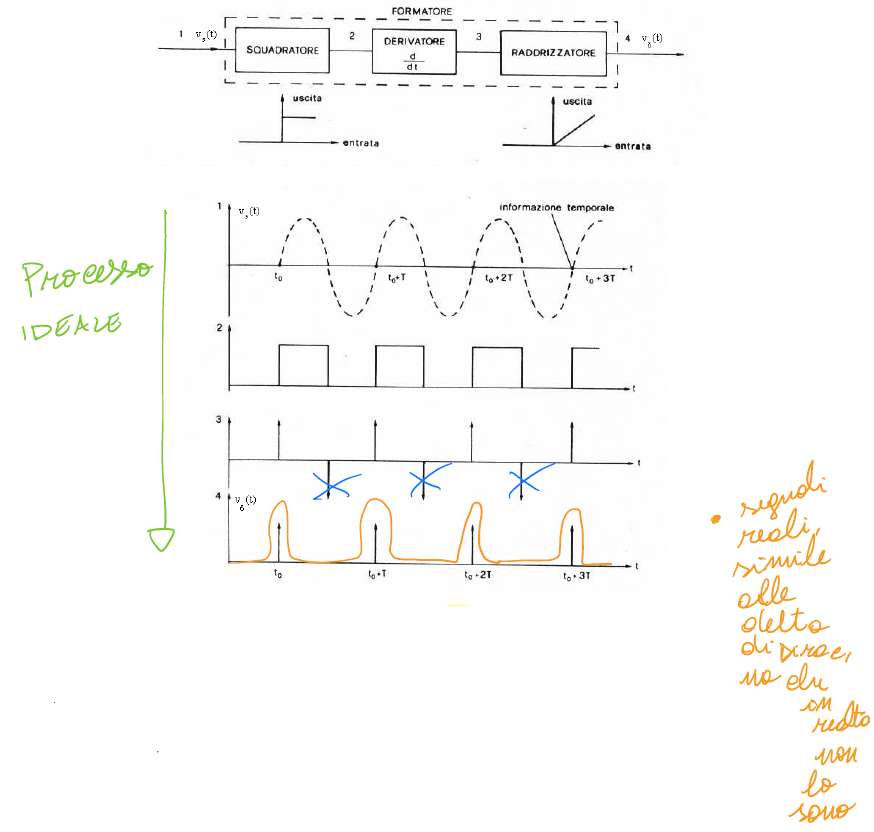
\includegraphics[scale = 1]{Recupero del segnale di clock schema.PNG}
\end{figure} 

\begin{tcolorbox}
    Se vuoi scoprire e andare a fondo su come è realizzato questo tipo di filtro, 
    ti rimando al corso di Misure Elettroniche in cui è spiegato il blocco FI Formatore di impulsi. \newline 

    \url{https://github.com/ciccio25/appunti-misure-elettroniche} \\
    Capitolo 12.3 - Frequenzimetro - blocco FI - pag 232 - 235 
\end{tcolorbox}

Nella pratica, realizzando il circuito di estrazione del sincronismo con componenti reali, 
esso potrà essere soltanto approssimato. \newline 

\newpage 

